\chapter{系统总体设计}\label{chap:design}

本章自顶向下介绍 Mood Radio 的总体架构、技术选型、数据模型与对外接口。系统遵循「\textbf{薄前端 + 厚后端 + 离线脚本}」的划分思路：所有耗时、需要长期记忆或与隐私强相关的能力下沉至 C++ 后端与 Python 离线脚本，前端只负责输入采集、可视化呈现与轻量级状态管理。

\section{总体架构}

系统由三层构成（\cref{fig:arch}）：浏览器中的 React 单页应用、本机运行的 C++ HTTP 服务，以及由后端按需拉起的 Python 子进程（用于音乐情绪分析与 LLM 代理）。三者通过 HTTP 与少量 SSE 通信，所有数据均落入本地的 \texttt{music\_mood.db}。

\begin{figure}[!htb]
  \centering
  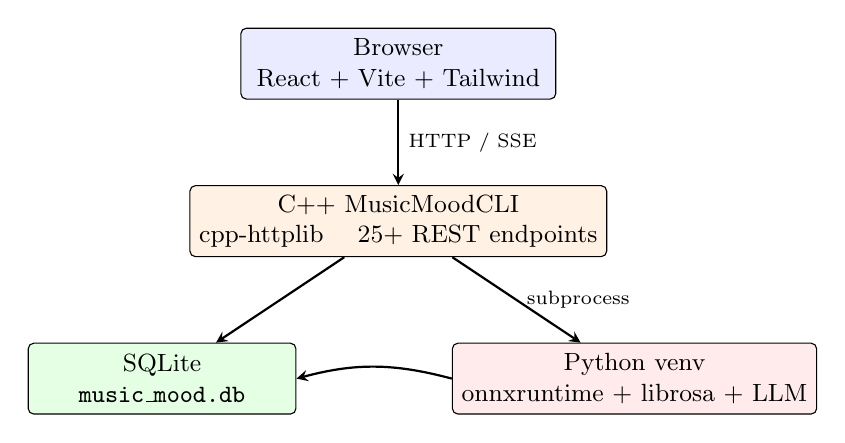
\begin{tikzpicture}[
      box/.style={draw, rounded corners=2pt, align=center,
        minimum width=4cm, minimum height=0.9cm, font=\small},
      arrow/.style={->, thick, >=stealth},
    ]
    \node[box, fill=blue!8] (fe) at (0, 4) {Browser \\ React + Vite + Tailwind};
    \node[box, fill=orange!10] (be) at (0, 2) {C++ MusicMoodCLI \\ cpp-httplib \quad 25+ REST endpoints};
    \node[box, fill=green!10, minimum width=3.4cm] (db) at (-3, 0) {SQLite \\ \texttt{music\_mood.db}};
    \node[box, fill=red!8, minimum width=3.4cm] (py) at (3, 0) {Python venv \\ onnxruntime + librosa + LLM};
    \draw[arrow] (fe) -- node[right, font=\scriptsize] {HTTP / SSE} (be);
    \draw[arrow] (be) -- (db);
    \draw[arrow] (be) -- node[right, font=\scriptsize] {subprocess} (py);
    \draw[arrow] (py.west) to[bend right=15] (db.east);
  \end{tikzpicture}
  \caption{Mood Radio 总体架构}\label{fig:arch}
\end{figure}

前端组件按页面切分，统一被一个全局的 \texttt{AppStateContext} 包裹，承担「曲库、人脸情绪、手动情绪、推荐歌单、情绪主题、心跳、时段、用户身份」等运行时状态的集中管理。后端以「单一可执行文件 + 内嵌 HTTP 服务」的方式发布，启动后即可对外提供包括「曲库扫描、播放历史、推荐生成、聊天代理、群体在场」等在内的 8 类 25 个以上的 REST 接口。

\section{技术栈与目录结构}

\subsection{技术选型}

\cref{tab:stack} 列出了系统主要的技术选型及其在本项目中的角色。

\begin{table}[!htb]
  \centering
  \caption{Mood Radio 技术选型}\label{tab:stack}
  \begin{tabularx}{\linewidth}{lX}
    \toprule
    \textbf{组件} & \textbf{用途} \\
    \midrule
    React 18 + Vite + TailwindCSS & 前端单页应用、路由与样式 \\
    Chart.js & 情绪四象限图与心情日志柱状图渲染 \\
    face-api.js & 浏览器端面部 7 类表情识别（本地推理） \\
    cpp-httplib & 后端 HTTP / SSE 服务（C++17 单文件） \\
    SQLite3 & 持久化（歌曲、播放历史、反馈、用户、在场） \\
    FFmpeg / FFTW / Eigen & 音频解码、Mel 频谱与张量计算 \\
    onnxruntime + librosa & Python 离线音乐情绪分析 \\
    nlohmann/json & 跨语言 JSON 序列化 \\
    \bottomrule
  \end{tabularx}
\end{table}

值得说明的是，最初实现采用 \texttt{ncnn} 作为 C++ 端的推理框架，但在实测中发现其输出范围严重失真，详见\cref{sec:onnx-fix}；最终通过引入 \texttt{onnxruntime + librosa} 的 Python 离线路径绕过该问题，得到了与训练时一致的 V/A 分布。

\subsection{目录结构（节选）}

为便于读者将本报告与代码仓库对应，\cref{lst:tree} 给出系统的关键目录结构。

\begin{lstlisting}[
  caption={Mood Radio 关键目录结构（节选）},
  label=lst:tree,
  basicstyle=\ttfamily\footnotesize,
  numbers=none,
  escapeinside={},
  mathescape=false,
  float=!htb,
]
Music_Mood_Detection/
|-- src/                       C++ 后端
|   |-- core/                  EmotionPredictor / AudioDecoder / FeatureExtractor
|   |-- db/DatabaseManager.h   8 张表 + 查询方法
|   |-- scanner/               worker pool + 文件登记
|   `-- server/WebServer.h     25+ endpoints (~1100 lines)
|-- scripts/                   Python 工具 (uv venv)
|   |-- analyze_all.py         onnxruntime 离线分析
|   `-- llm_chat.py            LLM 子进程代理
|-- frontend/web/              React + Vite + Tailwind
|   `-- src/{pages, components, hooks, contexts}/
|-- models/                    *.onnx + *.ncnn.*
|-- Music_Directory/.covers/   ID3 外置封面 (gitignored)
`-- start.ps1                  一键启动脚本
\end{lstlisting}

\section{数据模型}

\subsection{核心表设计}

系统采用 SQLite 作为本地存储，主体由 8 张表构成，关键表如\cref{tab:tables} 所示。

\begin{table}[!htb]
  \centering
  \caption{SQLite 关键表概览}\label{tab:tables}
  \begin{tabularx}{\linewidth}{lX}
    \toprule
    \textbf{表名} & \textbf{关键字段与用途} \\
    \midrule
    \texttt{tracks}        & \texttt{filepath, valence, arousal, duration, trajectory\_data, status}，歌曲主表 \\
    \texttt{directories}   & 用户监控的根目录 \\
    \texttt{play\_history} & \texttt{track\_id, played\_at, played\_pct, source}，全量播放日志，用于新鲜度评分 \\
    \texttt{user\_feedback}& \texttt{track\_id PK, kind}，喜欢/不喜欢，每曲一行可覆盖 \\
    \texttt{users}         & \texttt{uuid UNIQUE, nickname, created\_at}，匿名身份 \\
    \texttt{presence}      & \texttt{user\_id PK, mood\_label, valence, arousal, current\_track\_id, updated\_at}，实时心跳 \\
    \bottomrule
  \end{tabularx}
\end{table}

\subsection{关键索引}

考虑到推荐查询的频繁度，系统对情绪坐标与时间字段建立了如下索引：

\begin{lstlisting}[
  language=SQL,
  caption={SQLite 索引},
  label=lst:index,
  basicstyle=\ttfamily\footnotesize,
  float=!htb,
]
CREATE INDEX idx_va                ON tracks(valence, arousal);
CREATE INDEX idx_play_history_ts   ON play_history(played_at);
CREATE INDEX idx_presence_updated  ON presence(updated_at);
\end{lstlisting}

其中 \texttt{idx\_va} 服务于推荐时对二维坐标的范围查询，\texttt{idx\_play\_history\_ts} 用于在打分中快速回溯「最近 30 分钟 / 2 小时 / 6 小时 / 24 小时」内播放过的歌曲，而 \texttt{idx\_presence\_updated} 让群体在场页面能够在毫秒级完成 5 分钟时间窗内的聚合。

\section{对外接口}

后端对前端暴露的 REST 接口按功能划分为 8 类，重点接口如\cref{tab:api} 所示。SSE 端点 \texttt{/api/library/events} 用于实时推送扫描进度，避免前端轮询。

\begin{table}[!htb]
  \centering
  \caption{Mood Radio 主要 REST 接口（节选）}\label{tab:api}
  \begin{tabularx}{\linewidth}{llX}
    \toprule
    \textbf{方法} & \textbf{路径} & \textbf{用途} \\
    \midrule
    GET  & \texttt{/api/playlist/generate} & 按目标 V/A 与策略生成歌单（复合打分） \\
    GET  & \texttt{/api/tracks}            & 按象限/搜索条件获取曲库 \\
    POST & \texttt{/api/play\_history}     & 上报播放完成 \\
    POST & \texttt{/api/feedback}          & 上报喜欢/不喜欢 \\
    POST & \texttt{/api/chat}              & LLM 聊天代理 \\
    POST & \texttt{/api/user/register}     & 匿名用户注册 \\
    POST & \texttt{/api/presence}          & 心跳上报 \\
    GET  & \texttt{/api/presence/summary}  & 群体情绪聚合 \\
    GET  & \texttt{/api/library/events}    & SSE 扫描进度推送 \\
    \bottomrule
  \end{tabularx}
\end{table}
